

\chapter{Reinhardt domains and circular domains}\label{chap2}

\section{Reinhardt domains}\label{chap2:sec1}\pageoriginale

\begin{defi*}
A Reinhardt domain is an open set $\Omega \subset C^n$ such that 
$$
(z_1, \ldots, z_n) \epsilon \Omega \text{ implies } (e^{i\theta_1} z_1,
\ldots, e^{i\theta_n} z_n) \epsilon \Omega
$$
for all real $\theta_1, \ldots, \theta_n$.
\end{defi*}

\begin{thm}\label{chap2:thm1}
Let $\Omega \subset C^n$ be a connected Reinhardt domain containing 0
and suppose that $f(z)$ is holomorphic in $\Omega$, Then $f(z)$ can be
written 
$$
f(z) = \sum\limits_{m\epsilon N^n} a_m z^m
$$
in $\Omega$, the series converging normally in $\Omega$. Such an
expansion is unique.
\end{thm}

\begin{proof}
Let $\Omega_\epsilon$ be the set of $z \epsilon \Omega$ which have distance $>
\epsilon |z| (|z^2 = \sum |z_i|^2)$ from the boundary of $\Omega$. Let
$\Omega'_\epsilon \subset \Omega_\epsilon$ be the connected component of
$0$. Then
$$
\bigcup\limits_{\epsilon > 0} \Omega'_\epsilon = \Omega.
$$
For, if $z\epsilon \Omega$, we can join $z$ to the origin by a path in
$\Omega$. This path has a distance $>0$ from the boundary of
$\Omega$. If $\epsilon$ is small enough the path lies in $\Omega_\epsilon$ and
so in $\Omega'_\epsilon$. In particular, $z \epsilon \Omega'_\epsilon$.

Define, for $z\epsilon \Omega'_\epsilon$
$$
g(z_1,\ldots, z_n) = \frac{1}{(2\pi i)^n} \int\limits_{|t_1| = 1+\epsilon}
\ldots \int\limits_{|t_n| = 1+ \epsilon} \frac{f(t_1 z_1, \ldots, t_n
  z_n)}{(t_1-1) \ldots (t_n-1)} dt_1 \ldots dt_n. 
$$
The integral is defined, for if $(z_1, \ldots, z_n) \epsilon \Omega'_\epsilon$,
then $((1+\epsilon) z_1, \ldots, (1+\epsilon)z_n) \epsilon\Omega$ for
the distance 
between these two points is $\epsilon|z|$. Hence, since $\Omega$ is a
Reinhardt domain, $(t_1 z_1, \ldots, t_n z_n) \epsilon \Omega$ for all
$(t_1, \ldots, t_n)$ with $|t_j| = 1+ \varepsilon$. By differentiation
under the integral, it is seen that $g(z)$ is holomorphic in
$\Omega'_\varepsilon$. Moreover, if we choose\pageoriginale a polydisc
$K \subset \Omega'_\varepsilon$ with centre 0 such that $(1+\epsilon) K
\subset \Omega$, then for $z \epsilon \overset{\circ}{K}$, $(t_1 z_1,
\ldots, t_n z_n) \epsilon \Omega$ for all $|t_j|\leq 1+ \epsilon $ so that, by
Cauchy's formula, 
$$
g(z_1, \ldots , z_n) = f(z_1, \ldots, z_n), z \epsilon \overset{\circ}{K}. 
$$

Now, if two holomorphic functions in an open, connected set $U$
coincide in some open set in $U$, then they coincide in the whole of
$U$. (See the principle of analytic continuation in III). Hence
$$
f(z) = \frac{1}{(2\pi i)^n} \int\limits_{|t_1| = 1+ \epsilon} \ldots
\int\limits_{|t_n| = 1+ \epsilon }  \frac{f(t_1z_1, \ldots, t_n
  z_n)}{(t_1-1) \ldots (t_n -1)} dt_1 \ldots dt_n
$$ 
in $\Omega'_\epsilon$. Moreover,
$$
\frac{1}{(t_1-t) \ldots (t_n-1)} = \frac{1}{t_1 \ldots t_n}
\sum\limits_{(m_1,\ldots,m_n) \epsilon N^n} \frac{1}{t_1^{m_1}}  \ldots
\frac{1}{t_n^{m_n}} 
$$
the series being normally convergent on $|t_j| = 1 + \epsilon$, $j =
1,2,\ldots, n$. Hence
$$
f(z_1, \ldots , z_n) = \sum\limits_{(m_1, \ldots, m_n) \epsilon N^n}
\phi_{m_1 \ldots m_n} (z)
$$
where 
$$
\varphi_{m_1 \ldots m_n} (z) = \frac{1}{(2\pi i)^n} \int\limits_{|t_1|
= 1 + \epsilon} \ldots \int\limits_{|t_n|=1+\epsilon} \frac{f(t_1z_1, \ldots,
  t_n z_n)}{t^{m_1+1}_1 \ldots t^{m_n+1}_n} dt_1 \ldots dt_n. 
$$
Exactly as we proved above that $g(z) = f(z)$ in $\Omega'_\epsilon$, we
prove, using formula (3) for the derivatives of a holomorphic
function, that 
\begin{align*}
\phi_{m_1\ldots m_n} (z) & = \frac{1}{m_1 !\ldots m_n!}
\left. \frac{\partial^{ m_1 + \cdots m_n} f(t_1 z_1,\ldots, t_n
  z_n)}{\partial t^{m_1}_1 \ldots \partial t_n^{m_n}}\right| t_j=0 \\
& = \frac{z^{m_1}_1 \ldots z_n^{m_n}}{m_1!\ldots m_n!} \;
\frac{\partial^{ m_1+\cdots + m_n} f(0)}{\partial z_1^{m_1} \ldots
  \partial z_n^{m_n}}. 
\end{align*}

From\pageoriginale the integral representation of $\phi$, it is seen
that if $z$ lies in a compact subset $K\subset \Omega$ and $\epsilon$ is
small enough 
$$
|\phi_{m_1\ldots m_n} (z)| \leq \frac{M_K}{(1+\epsilon)^{m_1} \ldots
  (1+\epsilon)^{m_n}} 
$$
where $M_K$ depends only on $K$, so that the series converges normally
on $K$. The expansion in the whole of $\Omega$ follows easily by
letting $\epsilon\to 0$.

The uniqueness is obvious. 
\end{proof}

\section{Domains of convergence of powe series}\label{chap2:sec2}
Let
$$
\sum\limits_{m\epsilon N^n} a_m z^m
$$
be a given power series. We define its domain of convergence, $D$, as
follows: $z \epsilon D$ if the series converges absolutely in a
neighbourhood of $z$. $D$ is clearly open. We define the set $B$ as
the set of $z$ for which there exists $C>0$ such that $|a_m z^m| \leq
C$ for all $m \epsilon N^n$. Clearly $D \subset B^\circ$ (interior of
$B$). But we can prove that $D=B^o$. This follows from

\medskip
\noindent{\textbf{Abel's lemma:}}
If $z = (z_1, \ldots, z_n) \epsilon B$, then $(\alpha_1 z_1, \ldots,
\alpha_n z_n) \epsilon D$ if $|\alpha_1|<1, \ldots, |\alpha_n|<1$ and the
series converges normally in $D$. 

\begin{proof}
If $|a_m z^m| \leq C$, the general term of the series
$\sum\limits_{m\epsilon N^n} a_{m_1 \ldots m_n} \times$\break $(\alpha_1 z_1)^{m_1}
\ldots (\alpha_n z_n)^{m_n}$ is majorized by $C|\alpha_1|^{m_1} \ldots
|\alpha_n|^{m_n}$ and the result follows.
\end{proof}

\medskip
\noindent{\textbf{Consequences of Abel's lemma}}
\begin{itemize}
\item[(a)] $D = B^\circ$. This is obvious.

\item[(b)] The series represents a holomorphic function in $D$ (by I, Prop 2)

\item[(c)] $D$ is\pageoriginale a Reinhardt domain. More, if $(z_1,
  \ldots, z_n)$ then $(\alpha_1 z_1, \ldots,\break\alpha_n z_n)\epsilon D$ if
  $|\alpha_1| \leq 1, \ldots |\alpha_n| \leq 1$,  
\end{itemize}
and so $D$ is a union of polydiscs (all with centre).

We give an example, due to Hartogs, of a domain in $C^2$ that any
holomorphic function in the domain can be extended to a larger domain.

Let $G$ be the domain consisting of the points $z$ with
$$
|z_1| < \epsilon, \quad |z_2| < 1 
$$
and the points with 
$$
|z_1| < 1, \quad 1-\epsilon < |z_2| <1.
$$
In the figure we have indicated the variation in $|z_1|$, $|z_2|$. By
Theorem \ref{chap2:thm1}, any function holomorphic in $G$  can be
expanded in a power 
series in $G$ and, by Abel's lemma, the power series represents a
holomorphic function in the open polydisc
$$
|z_1| < 1, \quad |z_2| <1.
$$
\begin{figure}[H]
\centering
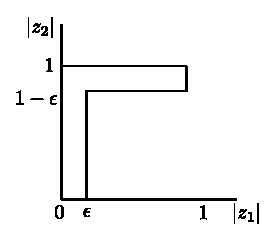
\includegraphics{figures/fig1.eps}
\end{figure}

A special case is the following:

Let $\Omega$ be an open set in $C^n(n>1)$ and $a$ a point of
$\Omega$. Let $f(z)$ be holomorphic in $\Omega -a$. Then $f(z)$ can be
continued holomorphically throughour $\Omega$.

Consequence (c) of Abel's lemma shows that the domain convergence of a
power series is a Reinhardt domain, but this is not\pageoriginale
all; not every Reinhardt domain, which is the union of open polydiscs, is the
domain of convergence of a power series. We can, however, characterize
the domains of convergence of power series.

Let $D^\ast \subset R^n$ be the set consisting of the points $(\log
|z_1|, \ldots, \log |z_n|)$ where $(z_1, \ldots, z_n) \epsilon D$
i.e. $D^\ast$ is the image of $D$ under the mapping $\phi : C^n \to
R^n$ defined by $\phi(z_1,\ldots, z_n) = (\log |z_1|, \ldots, \log
|z_n|)$. Let $B^\ast$ be  the image of $B$ under $\phi$ ($D$ and $B$
are the sets of points defined on p.11 associated with the power
series). If $(\rho_1, \ldots, \rho_n)\epsilon D^\ast$ then $(\rho_1 - t_1 ,
\ldots, \rho_n - t_n) \epsilon D^\ast$ if $t_1 \geq 0, \ldots, t_n \geq 0$.

The following fundamental result holds. 

\begin{thm}\label{chap2:thm2}
$D^\ast$ is a convex set in $R^n$.
\end{thm}

\begin{proof}
Since $D=B^0$, $D^\ast = \overset{\circ}{B^\ast}$ so that it suffices
to prove that $B^\ast$ is convex. Now $B^\ast = \bigcup\limits_{C>0}
B^\ast_C$, where $B^\ast_C$ is the image, under $\phi$, of the set of
$z\epsilon C^n$ where $|a_m z^m| \leq C$ for all $m \epsilon N^n$. Since
$B^\ast_C \subset B^\ast_{C'}$, if $C<C'$ it is enough to prove that
$B^\ast_C$ is convex. Also $B^\ast_C = \bigcap\limits_{m\epsilon N^n}
B^\ast_{C,m}$, where $B^\ast_{C,m}$ is the image of the set of $z\epsilon
C^n$, $|a_m z^m| \leq C$ for a fixed $m$, under $\phi$. Thus, we have
only to prove that $B^\ast_{C,m}$ is convex. Now $B^\ast_{C,m}$ is the
image of the set of $z \epsilon C^n$ for which $\left|a_{m_1 \ldots m_n}
z_1^{m_1} \ldots z^{m_n}_{n} \right| \leq C$ and so is the set of
points $(\rho_1, \ldots , \rho_n) \epsilon R^n (\rho_j = \log |z_j|)$ at
which 
$$
\log |a_{m_1 \ldots m_n}| + m_1 \rho_1 + \cdots + m_n \rho_n \leq \log
C, 
$$
which, being a half space in $R^n$, is convex. This proves Theorem
\ref{chap2:thm2}. 

For\pageoriginale example, consider a series convergent in the domain
in $C^2$ consisting of the points $|z_1| <1$, $|z_2| <e$, and the
points $|z_1| < e$, $|z_2|<1$. It has the image shown in Fig. (a) (the
set $\alpha$) in the $(|z_1|, |z_2|)$-plane and $D^\ast$ contains the
set $\alpha^\ast$ in Fig. (b). Since $D^\ast$ is convex, it contains
also the set $\beta^\ast$ in Fig. (b) and so the series converges at
the points in $C^2$ which are mapped by 
$$
\phi : z \to (\log |z_1|, \log |z_2|) 
$$
into the set $\beta'$ in Fig. (a).

\begin{figure}[H]
\centering
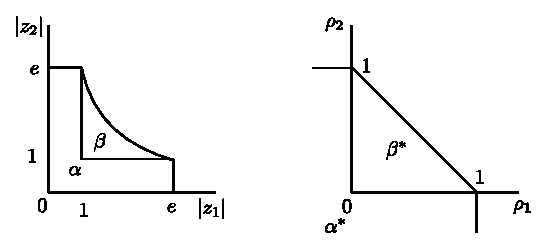
\includegraphics{figures/fig2.eps}
\centerline{\textbf{Fig. (a)} \hspace{3cm} \textbf{Fig. (b)}}
\end{figure}

The converse of Theorem \ref{chap2:thm2} is true; that is if a Reinhardt domain,
which is the union of polydiscs, is such that its image under $\phi$
is convex, then it is (precisely) the domain of convergence of a power
series. We shall prove this later (in VII, p.44)
\end{proof}

\section{Circular domains}\label{chap2:sec3}
We consider next the expansion of holomorphic functions in series of
homogeneous polynomials. 

\begin{defi*}
An open set $\Omega \subset C^n$ is said to be a \textit{circular
  domain} if $z \epsilon \Omega$ implies\pageoriginale $e^{i\theta} z\epsilon
\Omega$ i.e. $(e^{i\theta} z_1 , \ldots, e^{i\theta} z_n) \epsilon \Omega$
for all real $\theta$.
\end{defi*}

\begin{thm}\label{chap2:thm3}
Let $\Omega$ be a connected circular domain and let $0
\epsilon\Omega$. Suppose $f(z)$ to be holomorphic in $\Omega$. Then $f(z)$
can be expanded in a series of homogeneous polynomials,
$$
f(z) = \sum\limits^\infty_{k=0} P_k (z) \text{ in } \Omega
$$
($P_k(z)$ is homogeneous, of degree $k$ in $z_1, \ldots, z_n$) and the
series converges normally in $\Omega$. An expansion of this form is
unique. 
\end{thm}

\begin{proof}
Define $\Omega'_\epsilon$ as in Theorem \ref{chap2:thm1} and consider
the integral  
$$
\frac{1}{2\pi i} \int\limits_{|t| = 1 + \epsilon} \frac{f(t z_1, \ldots,
  tz_n)}{t-1} \; dt. 
$$
Exactly as in the proof of Theorem \ref{chap2:thm1}, we choose a polydisc $K$ about
the origin such that $(1+\epsilon) K \subset \Omega'_\epsilon$ and then, if $z
\epsilon K$, $(t z_1, \ldots, tz_n) \epsilon \Omega$ for $|t| \leq 1$ so that,
the integral being holomorphic in $\Omega'_\epsilon$ we have, by Cauchy's
formula, 
$$
f(z_1, \ldots, z_n) = \frac{1}{2 \pi i} \int\limits_{|t| = 1+\epsilon}
\frac{f(tz_1, \ldots, tz_n)}{t-1} dt.
$$
in $\overset{\circ}{K}$ and so, since $\Omega'_\epsilon$ is connected, in
$\Omega'_\epsilon$. Since
$$
\frac{1}{t-1} = \frac{1}{t} \sum\limits^\infty_{k=0} \frac{1}{t^k}, 
$$
the series converging normally on $|t| = 1+ \epsilon$, we have
$$
f(z_1, \ldots, z_n) = \sum\limits^\infty_{k=0} P_k(z)
$$
where
$$
P_k (z) = \frac{1}{2\pi i} \int\limits_{|t|=1+\epsilon} \frac{f(tz_1,
  \ldots, tz_n)}{t^{k+1}} \; dt.
$$\pageoriginale
As in the proof of Theorem \ref{chap2:thm1}, the series converges normally in
$\Omega'_\epsilon$ and, repeating the above argument, it follows that 
\begin{gather*} 
P_k (z) = \frac{1}{k!} \left|\frac{d^k f(t z_1, \ldots, tz_n)}{}
\right|_{t=0} \\
= \frac{1}{k!} \sum\limits_{m_1 + \cdots + m_n = k} \frac{\partial^k
  f(0)}{\partial^{m_1} z_1 \ldots z^{m_n}_n} z^{m_1}_1 \ldots z^{m_n}_n
\end{gather*}
The theorem follows by letting $\epsilon \to 0$.

It is easily seen that if $f(z)$ has an expansion
$\sum\limits^\infty_{k=0}P_k (z)$ which converges uniformly in a
neighbourhood of $0$, then $P_k (z)$ has the above form. This proves
Theorem \ref{chap2:thm3}. 

The above theorem shows that if a function $f(z)$ is holomorphic is a
circular domain $\Omega$ (which is connected and contains 0) then it
can be holomorphically continued to $\bigcup\limits_{0\leq t \leq 1}
(t\Omega)$. This is proved in the same way as Abel's lemma. 
\end{proof}
